\documentclass[12pt,a4paper,polish]{article}
\topmargin -1.6cm
\addtolength{\textheight}{4cm}
\textwidth  15.5cm

\leftmargin      5mm
\rightmargin     5mm
\oddsidemargin   5mm
\evensidemargin  5mm

\usepackage{hyperref}
\usepackage{polski}
\usepackage[utf8]{inputenc}
\usepackage{graphicx} % To jest pakiet do grafiki.
                      % Moze przydac sie pozniej.
\usepackage{units}
\usepackage{sty/wds}


\wdsTytulProjektu{RoboVision}
\wdsAutor{Marcin Bober, 249426}




\begin{document}
%
% To po to, aby mieć format A4.
% pdflatex domyślnie tworzy dokument w formacie letter.
%
\pdfpageheight   297mm
\pdfpagewidth    210mm

\wdsStronaTytulowa
\wdsSpisTresci


 \section{Charakterystyka tematu projektu}
 \label{sekcja-charakterystyka}

  Projekt ma na celu stworzenie aplikacji okienkowej, która poprzez połączenie
  internetowe będzie w stanie wydawać polecenia do robota mobilnego, sterować nim,
  a także pobierać informacje z czujników i wizualizować je.

 \section{Podcele i etapy realizacji projektu}

  Projekt powdzielony będzie na kilka pomniejszych celów tak, aby każdy z nich
  mógłbyć osobno rozwijany. \\

  Lista podelów:
  \begin{itemize}
    \item Zapoznanie się z dostępną literaturą związaną z tematem oraz zdobycie 
    informacji niezbędnych do zrealizowania zadania.
    \item Przygotowanie graficznego szkicu aplikacji wraz z rozplanowaniem funkcionalności.
    \item Zdefiniowanie protokołu komunikacyjnego, struktury ramek przesyłanych danych
     i implementacja interfejsu sieciowego.
    \item Parsowanie danych odbieraych z robota.
    \item Przygotowanie wizualizacji zebranych danych.
    \item Obsługa klawiatury i joysticka.
    \item Implementacja algorytmu sterowania i przesyłanie wyników do urządzenia.
  \end{itemize}

 \section{Specyfikacja finalnego produktu}

    % Jakie są spodziewane efekty realizowanego projektu.
    % Jakie są oczekiwane zakresy mierzonych wartości, dokładności itp.
  Aplikacja będzie w stanie wizualizować dane odbierane z czujników robota.
  Będą to między innymi:
  \begin{itemize}
    \item wskazania akcelometru,
    \item wskazania żyroskopu,
    \item aproksymacja poziomu baterii,
    \item odlegość przeszkody zczytanej z przedniego czujnika ultradzwiękowego,
    \item prędkość rzeczywista pojazdu z enkoderów.
  \end{itemize}
  

  \newpage
  \section{Terminarz realizacji poszczególnych podcelów 
     {\small (z dokładnością do 1 tygodnia)}}

  \begin{itemize}
    \item 22 marca 2020  -- zakończenie przeglądu materiałów
                            związanych z danym tematem
    \item 29 marca 2020 -- przygotowanie schematu widoku aplikacji
    \item 12 kwietnia 2020 -- oprogramowanie obsługi joysticka
    \item 19 kwietnia 2020 -- zdefiniowanie szczegółów komunikacji i budowy przesyłanych ramek
    \item 26 kwietnia 2020 -- przygotowanie logiki sterownia
    \item  4 maja 2020 -- implementacja dwustronnej komunikacji z robotem
    \item 10 maja 2020 -- wizualizacja wskazań prędkości i naładowania baterii
    \item 17 maja 2020 -- wizualizacja wskazań akcelometru
    \item 24 maja 2020 -- przygotowanie wizualizacji obiektu 3D
    \item 31 maja 2020 -- implementacja obracania obiektu 3D przy użyciu żyroskopu
    \item  7 czerwca 2020 -- Szukanie błędów i testowanie wszystkich funkcji
    \item 14 czerwca 2020 -- Ostateczne testy działania aplikacji
  \end{itemize}
  %
  % Dopełnieniem harmonogramu powinien być diagram Gantta.

  \begin{figure}[ht]
    \centering
    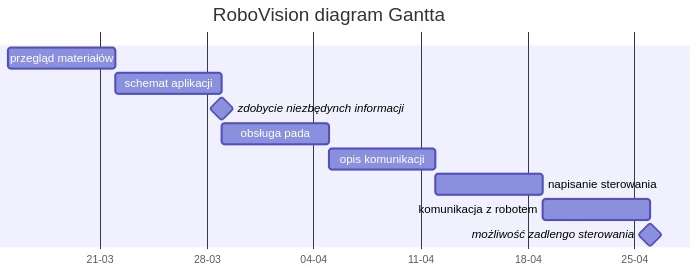
\includegraphics[width=1\textwidth]{gantt.jpg}
    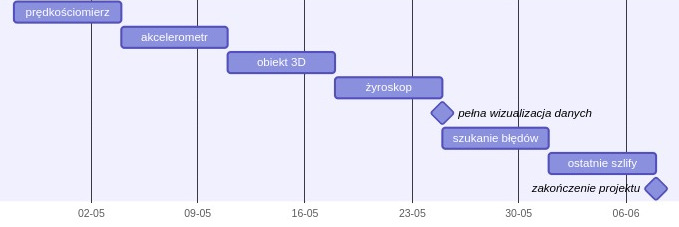
\includegraphics[width=1\textwidth]{gantt2.jpg}
    \caption{Diagram Gantta}
    \label{fig:ogniwa}
  \end{figure}




% \section{{\it Kilka przykładów wykorzystania \LaTeX a} }

%  To rozdział jest tu tylko po to, aby zaprezentować wybrane
%  możliwości \LaTeX a.
%  Przy odwoływaniu się do rozdziałów zawsze stosujemy odwołanie
%  przez etykietę. Nigdy nie odwołujemy się wpisując konkretny
%  numer, np. tutaj wykorzystując polecenie {\tt $\backslash$ref}
%  można odwołać się do rozdziału \ref{sekcja-charakterystyka}.
%  Można też podać stronę, na której ten rozdział jest, 
%  np. patrz rodział  \ref{sekcja-charakterystyka} 
% (str.  \pageref{sekcja-charakterystyka}).
%  Przy małych dokumentach to nie ma sensu, ale może się przydać
%  przy większych.

%  W ten sam sposób odwołujemy się do równań i wzorów,
%  \begin{equation}
%     F = ma
%   \label{wzor-Newton2}
%  \end{equation}
%  np. możemy wskazać równianie (\ref{wzor-Newton2}).
%  \begin{figure}[hbpt]
%    \center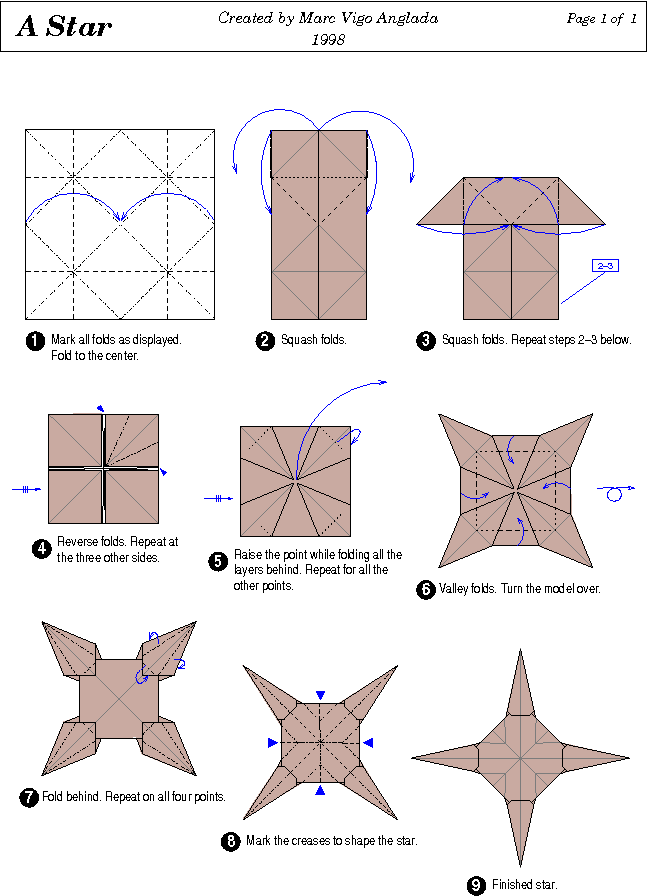
\includegraphics[width=6cm]{img/origami-gwiazda.png}
%    \caption{Podpis pod rysunkiem.}
%    \label{rysunek-gwiazda}
%  \end{figure}
%  W analogiczny sposób odwołujemy się do rysunków, tak
%  jak np. do rys. \ref{rysunek-gwiazda} (Uwaga: etykieta musi
%  być zdefiniowana po instrukcji {\tt $\backslash$caption}).

%  Literaturę należy cytować dowołując się do pozycji 
%  z bazy biliograficznej (jest ona w podkartotece {\tt bib}
%  w pliku {\tt  baza\_bibliografii.bib}.
%  Odwołujemy się również do nich również poprzez etykiety
%  np. \cite{HTTP2}\cite{Hallam:PHD-thesis}
%  lub \cite{Blanchette:Qt}. Etykietą jest
%  pierwszy element w danej pozycji biliograficznej.


% \section{Przykłady zapisu jednostek z wykorzystaniem pakietu {\sf units}}

% Opis pakietu: {\tt https://ctan.org/pkg/units}\\[1ex]
% \begin{tabular}{rcl}
%   Odległość/długość & -- & \unit[2,4]{m}             \\[1ex]
%   Szybkość          & -- & \unitfrac[48]{km}{h}      \\[1ex]
%   Szybkość          & -- & \unit[48]{$\frac{km}{h}$} \\[1ex]
%   Napięcie          & -- & \unit[$-5$]{V}, \unit[$+12$]{V} \\[1ex]
%   Kąt               & -- & 15$^\circ$
% \end{tabular} 

\bibliographystyle{plplain}
\bibliography{baza_bibliografii}
\end{document}

